\thispagestyle{toanhocvadoisongnone}
\pagestyle{toanhocvadoisong}
\everymath{\color{toanhocdoisong}}
\graphicspath{{../toanhocdoisong/pic2/}}
\blfootnote{$^1$\color{toanhocdoisong}Hà Nội.}
\begingroup
\AddToShipoutPicture*{\put(0,616){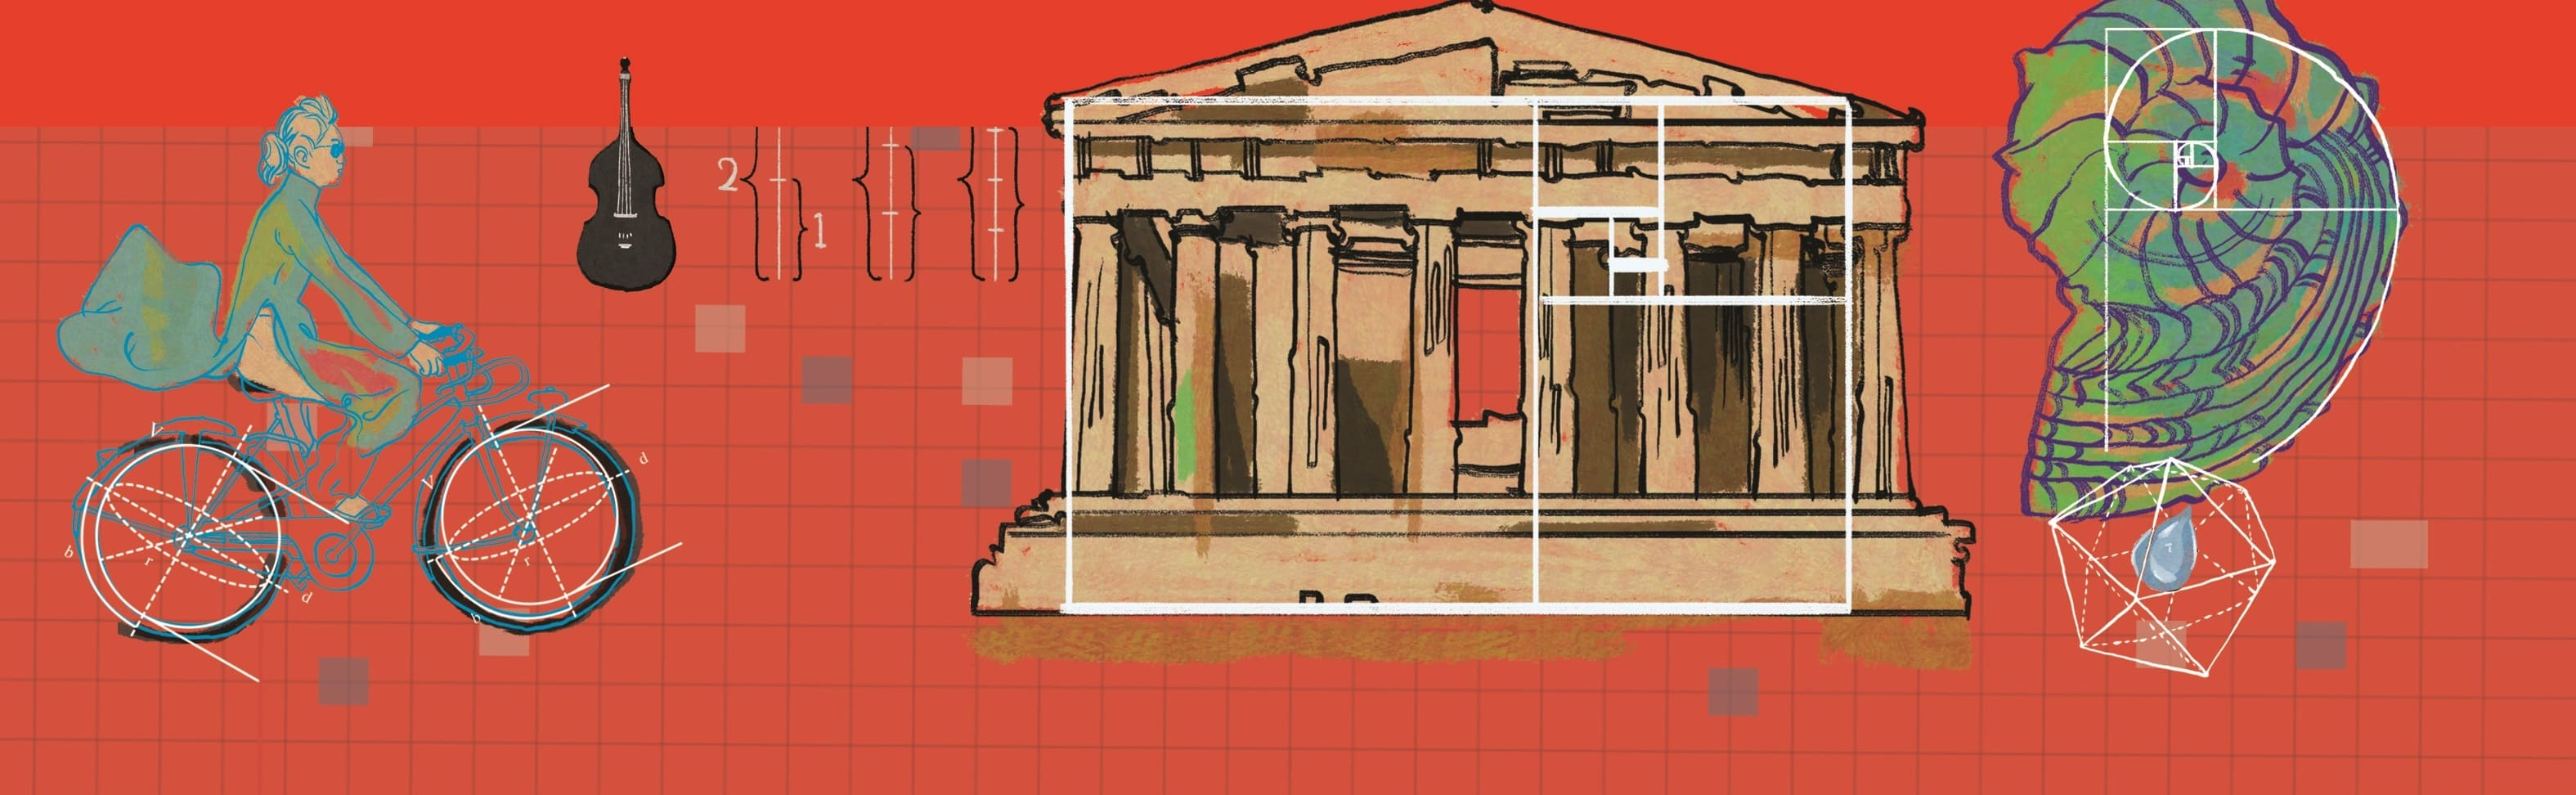
\includegraphics[width=19.3cm]{../bannertoanhocdoisong}}}
\AddToShipoutPicture*{\put(137,523){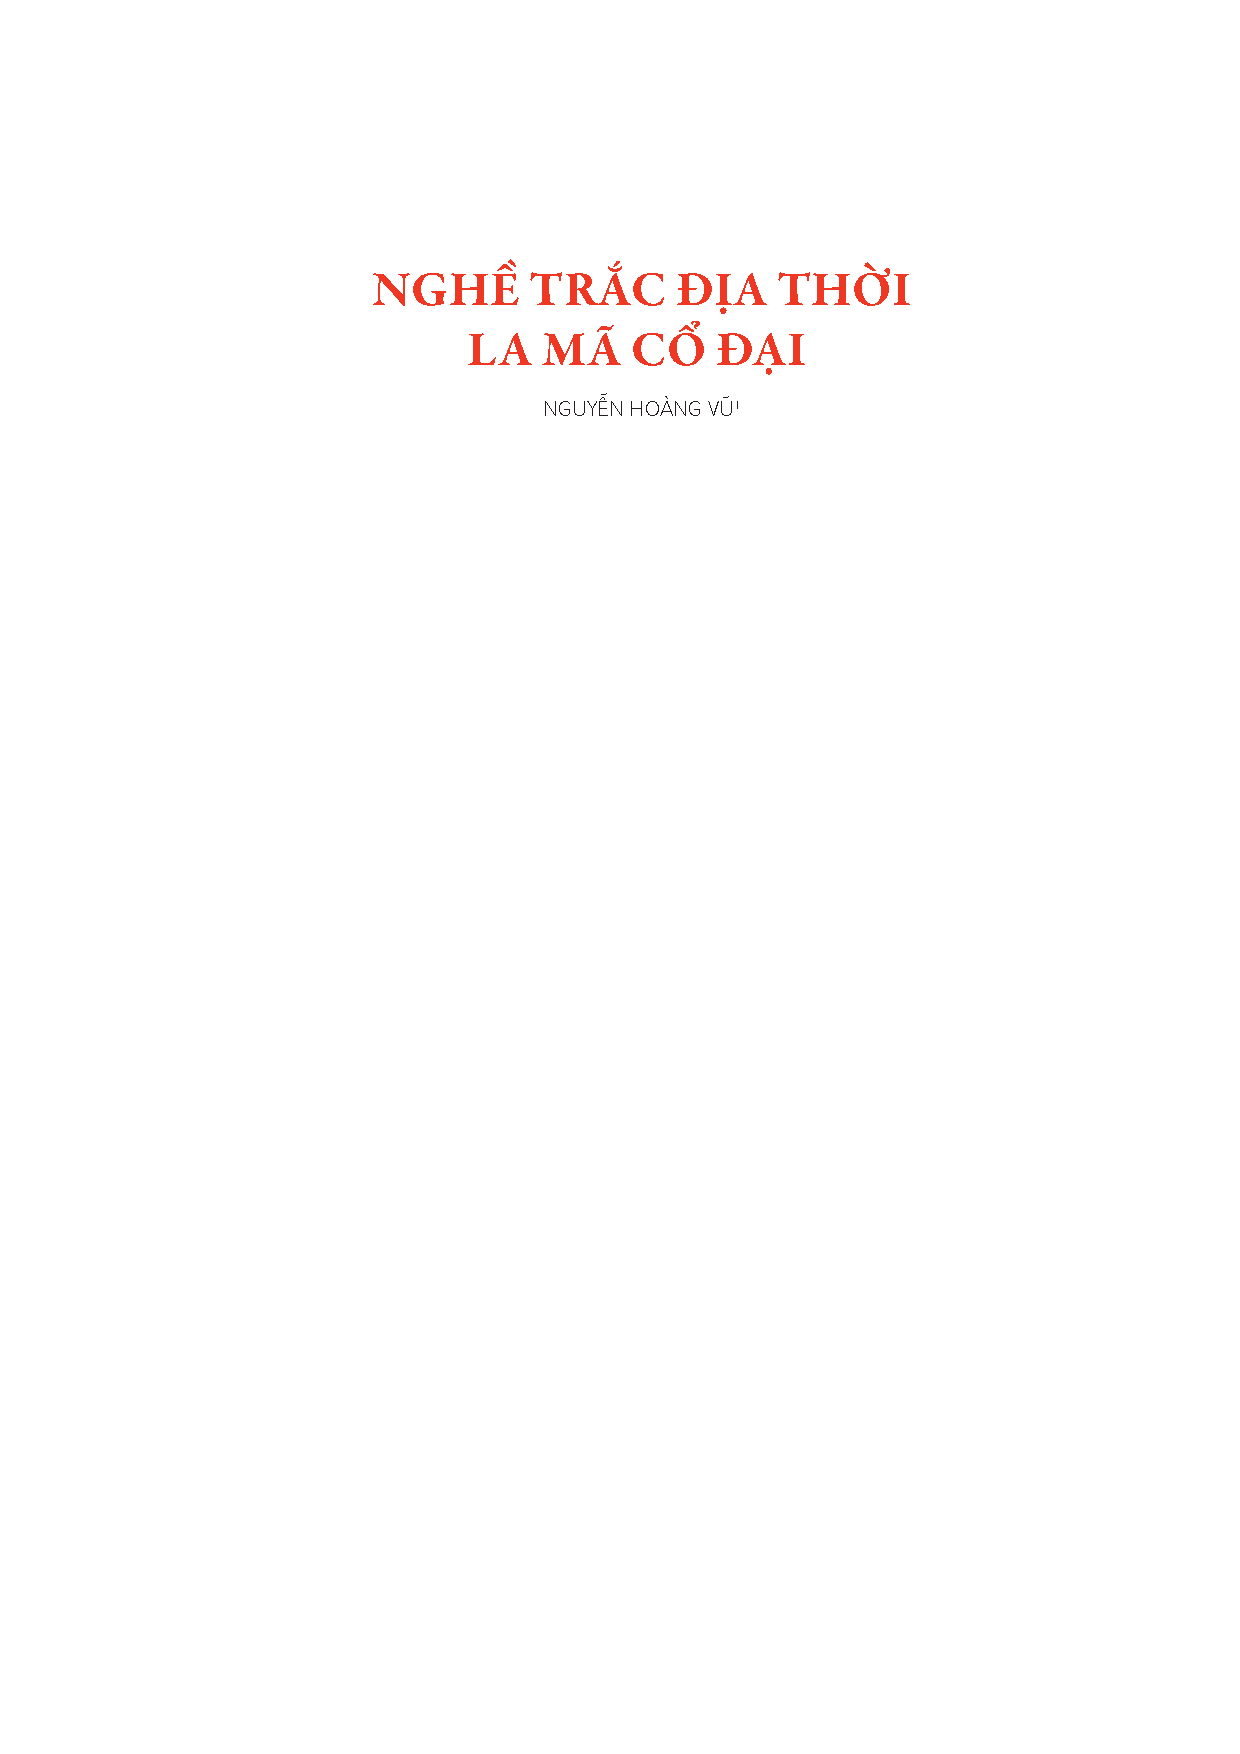
\includegraphics[scale=1]{../tieude2.pdf}}}
\centering
\endgroup

\vspace*{185pt}
\begin{multicols}{2}
	Gắn liền với sự phát triển của hình học, nghề trắc địa cũng xuất hiện rất sớm trong lịch sử nhân loại, từ nhiều nghìn năm trước. Đặc biệt, đến thời La Mã cổ đại, nó đóng một vai trò quan trọng trong nhiều mặt của xã hội. Trong bài viết này, chúng ta hãy cùng tìm hiểu về các công cụ và phương pháp đo đạc cũng như những thành tựu còn lưu lại của trắc địa La Mã.
	\vskip 0.1cm
	$\pmb{1.}$ \textbf{\color{toanhocdoisong}Các dụng cụ trắc địa}
	\begin{figure}[H]
		\vspace*{-5pt}
		\centering
		\captionsetup{labelformat= empty, justification=centering}
		
\includegraphics[height=0.8\linewidth]{1a}
		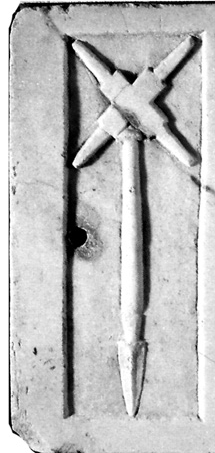
\includegraphics[height=0.8\linewidth]{1b}
		\caption{\small\textit{\color{toanhocdoisong}Hình $1$. Hình khắc groma trên bia mộ của những người làm trắc địa thời La Mã.}}
		\vspace*{-10pt}
	\end{figure}
	Ngoài các dụng cụ cơ bản thường thấy như cọc và dây thừng, dụng cụ trắc địa mang tính biểu tượng nhất của người La Mã là một thiết bị mang tên \textit{groma}. Nó xuất hiện phổ biến trong nhiều tài liệu trắc địa còn sót lại cũng như trên bia mộ của những nhà trắc địa La Mã. Từ hiện vật phát hiện được ở di chỉ Pompeii và các mô tả bằng lời trên văn bản, cấu tạo của thiết bị này gồm một số bộ phận chính như sau:
	\vskip 0.1cm
	$\bullet$ Một thân chính dạng cọc;
	\vskip 0.1cm
	$\bullet$ Một thanh chữ thập gắn lên thân chính;
	\vskip 0.1cm
	$\bullet$ Bốn dây dọi gắn ở bốn đầu của thanh chữ thập.
	\begin{figure}[H]
		\vspace*{-5pt}
		\centering
		\captionsetup{labelformat= empty, justification=centering}
		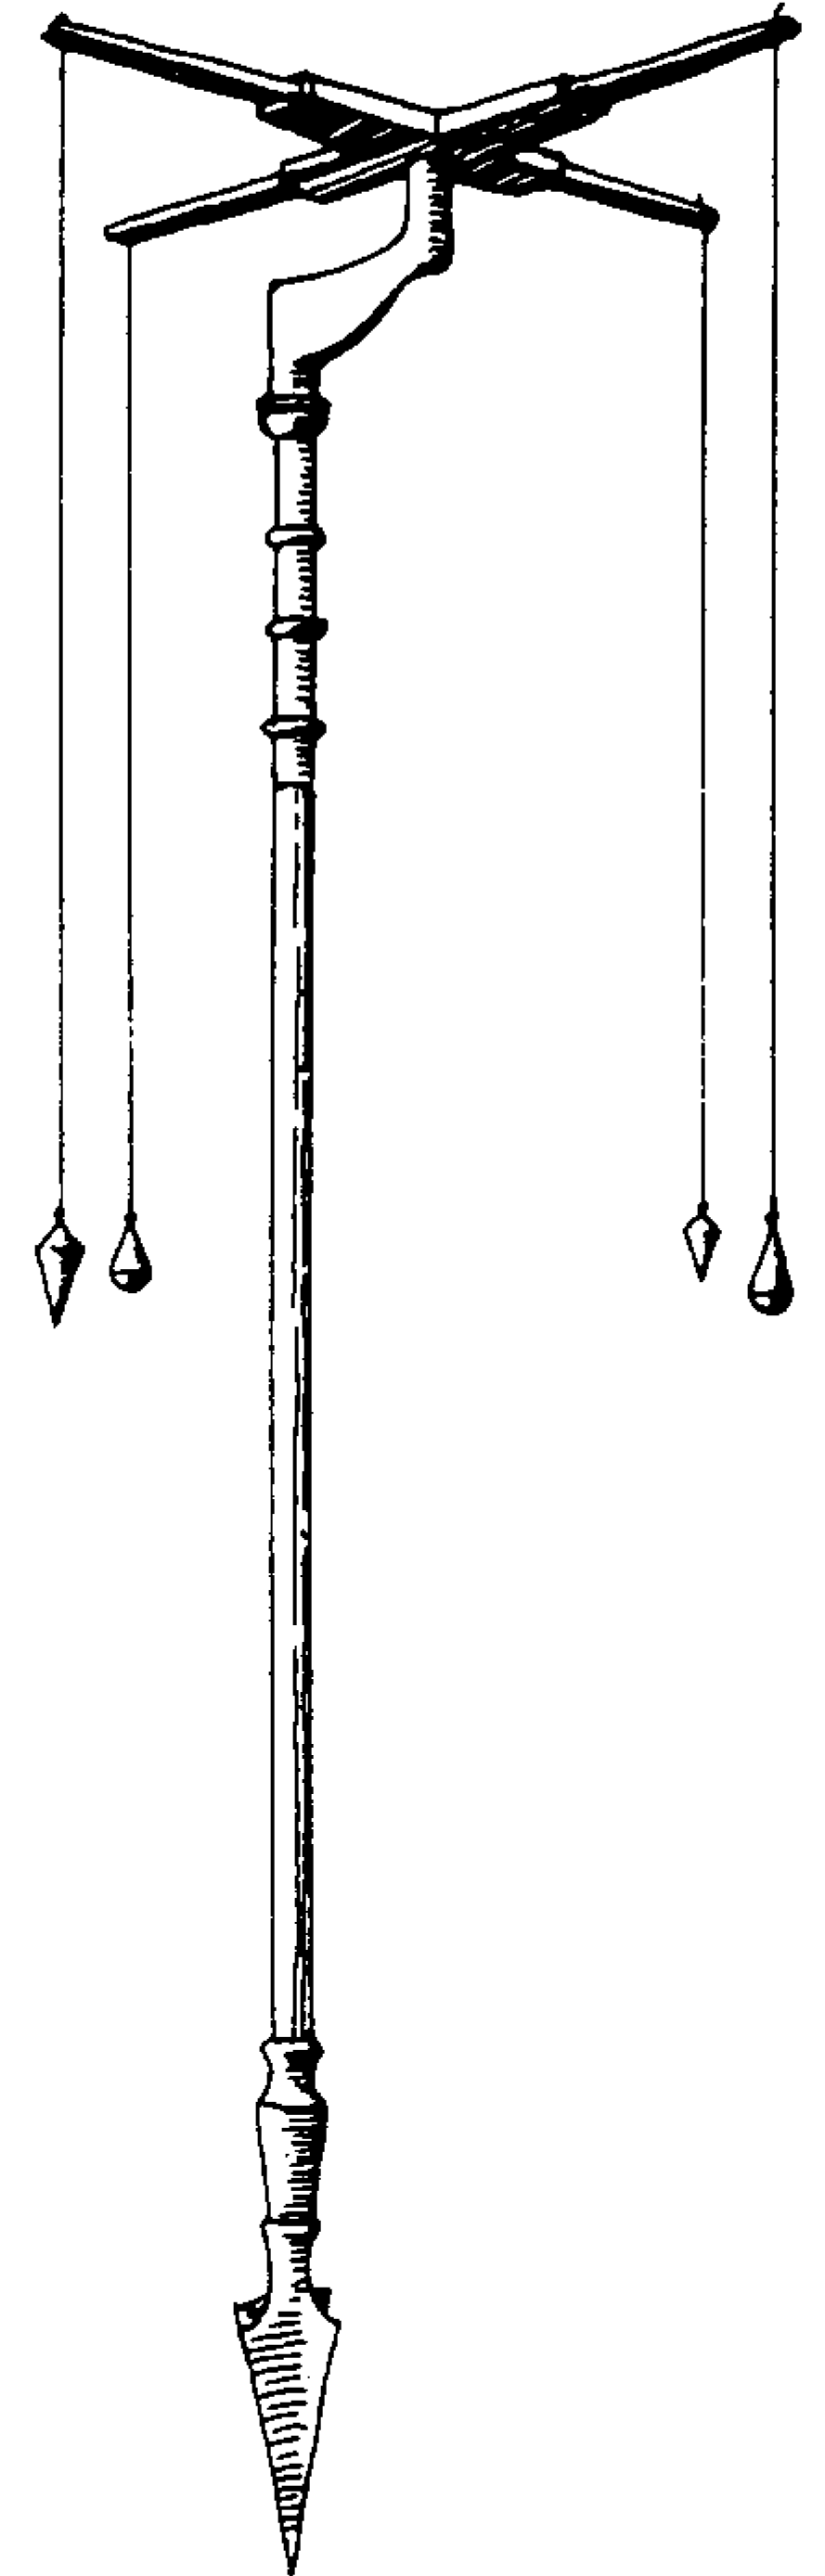
\includegraphics[height=0.8\linewidth]{2a}
		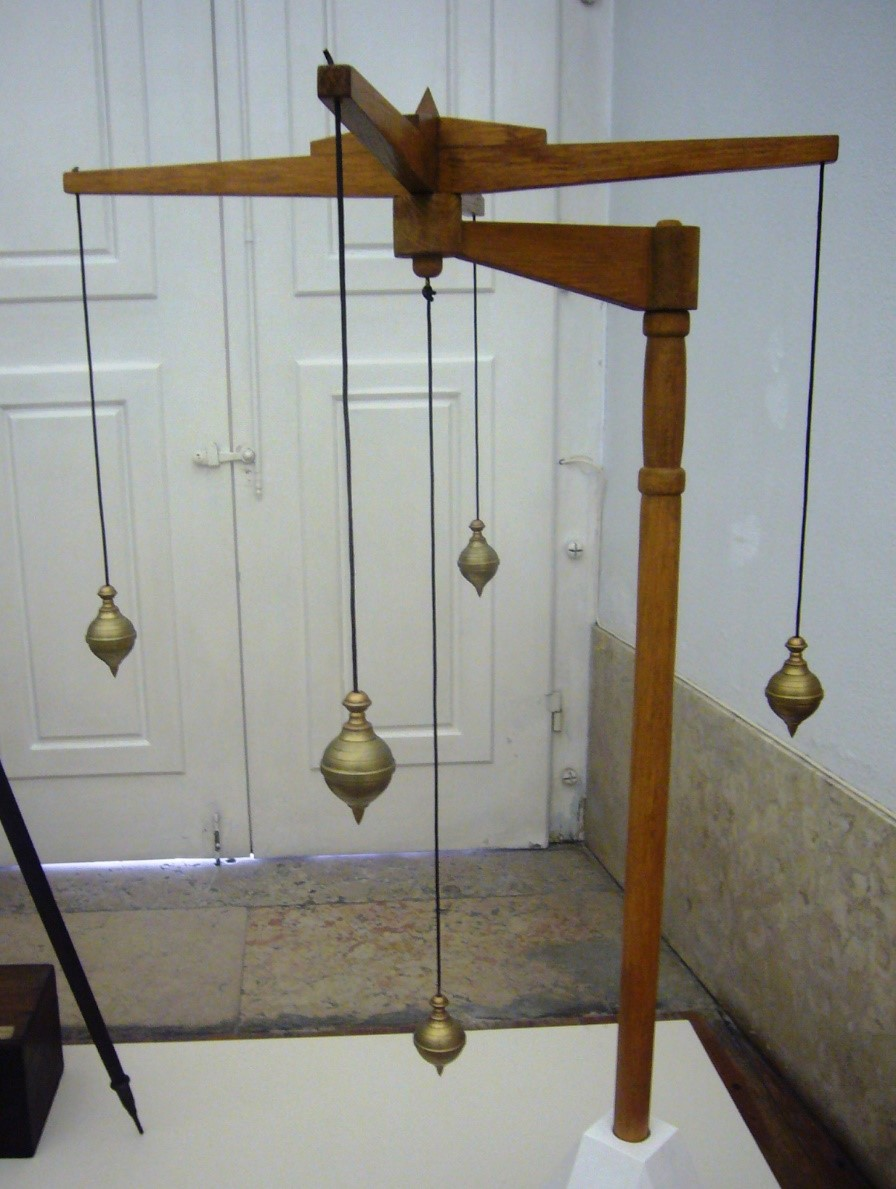
\includegraphics[height=0.8\linewidth]{2b}
		\caption{\small\textit{\color{toanhocdoisong}Hình $2$. Sơ đồ cấu tạo của groma (trái) và một phiên bản phục dựng (phải).}}
		\vspace*{-10pt}
	\end{figure}
	Việc sử dụng \textit{groma} để xác định góc vuông tương đối đơn giản. Thân chính được cắm sao cho hai dây dọi của một nhánh chữ thập  thẳng hàng với các cọc đã được cắm sẵn. Sau đó người ta cắm thêm các cọc mới gióng hàng với hai dây dọi của nhánh chữ thập còn lại để xác định phương vuông góc.
	\begin{figure}[H]
		\vspace*{-5pt}
		\centering
		\captionsetup{labelformat= empty, justification=centering}
		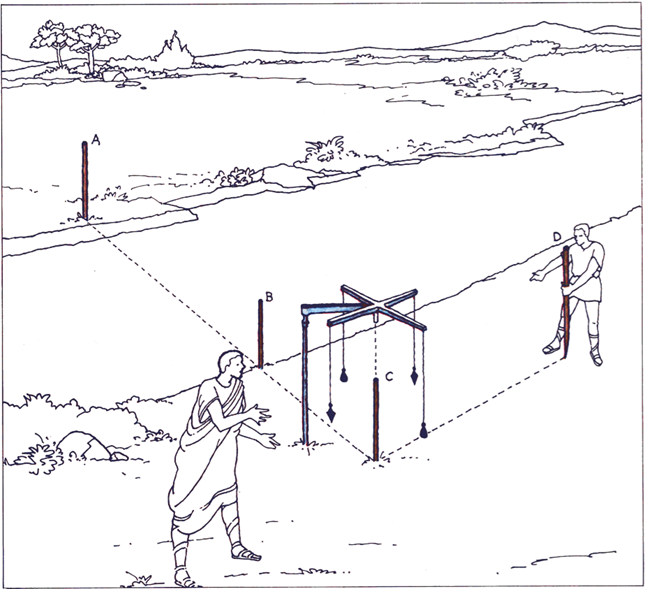
\includegraphics[width= 1\linewidth]{3}
		\caption{\small\textit{\color{toanhocdoisong}Hình $3$. Minh họa cách sử dụng groma để xác định phương vuông góc với một phương cho trước.}}
		\vspace*{-10pt}
	\end{figure}
	Về mặt lịch sử, người Ai Cập cổ đại cũng đã có một thiết bị trắc địa gần giống với \textit{groma}. Một số giả thuyết cho rằng \textit{groma} được du nhập vào xã hội La Mã từ người Etruria, những người sống ở khu vực phía bắc của Italy trước khi bị người La Mã sáp nhập, kèm theo đó là các nghi thức mang màu sắc tôn giáo khi sử dụng công cụ này. Do việc đo đạc xác định biên giới các công trình còn có ý nghĩa về mặt tâm linh (giống với ``động thổ" của nước ta) nên trong giai đoạn ban đầu của đế quốc La Mã, những người làm trắc địa có vai trò giống với các giáo sỹ hơn là nhân viên kỹ thuật và \textit{groma} là một biểu tượng nghi lễ gắn liền với công việc này. Dần dần, trắc địa trở thành nghề nghiệp mang tính dân sự và mất đi màu sắc huyền bí của nó.
	\vskip 0.1cm
	Bản thân \textit{groma} cũng có nhiều vấn đề về mặt kỹ thuật. Nó không thể sử dụng được khi có gió, ngay cả với gió nhẹ, do các dây dọi không còn thẳng đứng nữa. Nhà toán học Heron ở Alexandria cũng đã nhắc đến việc này. Ông đề xuất thêm các lá chắn gió cho các dây dọi nhưng cũng nhận định rằng việc này sẽ làm cho quá trình gióng hàng khó khăn hơn nhiều. Mặt khác, \textit{groma} cũng cho độ chính xác không cao. Với khoảng cách $100$ m, độ lệch của việc gióng hàng so với đường thẳng cần tìm có thể lên tới $1$ m. Một số tác giả như Jean--Pierre Adam cho rằng các bước gióng hàng liên tiếp sử dụng \textit{groma} sẽ triệt tiêu bớt sai số do ở mỗi bước do kết quả đo sẽ lệch sang trái hoặc phải một cách ngẫu nhiên. Trong khi đó, một số nhà nghiên cứu khác lại cho rằng \textit{groma} chỉ mang tính biểu tượng còn các công cụ chính của người làm trắc địa La Mã là những thiết bị chính xác hơn.
	\begin{figure}[H]
		\vspace*{-5pt}
		\centering
		\captionsetup{labelformat= empty, justification=centering}
		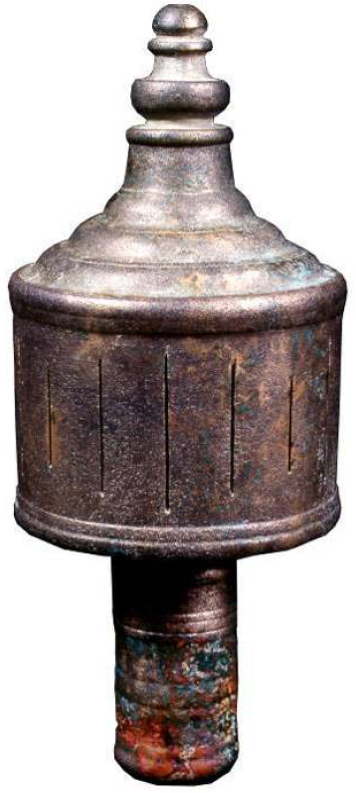
\includegraphics[width= 0.4\linewidth]{4}
		\caption{\small\textit{\color{toanhocdoisong}Hình $4$. Đầu ngắm từ thời La Mã được khai quật ở Pháp.}}
		\vspace*{-10pt}
	\end{figure}
	Năm $1997$, cuộc khai quật một di chỉ La Mã ở Pháp phát hiện một đầu ngắm hình trụ với các khe cách nhau $1/16$ đường tròn. Trước đó, người ta cũng đã phát hiện được ở Đức một dụng cụ có khe ngắm tương tự dạng bát giác (hiện vật này đã bị mất trong chiến tranh thế giới thứ hai). Điều đáng chú ý là đầu ngắm dạng này có thể cho phép xác định phương vuông góc hoặc các góc $1/4$, $1/8$ hay $1/16$  đường tròn với độ chính xác cao hơn nhiều so với \textit{groma}. Sau thời La Mã, chúng chỉ xuất hiện lại và phổ biến ở châu Âu vào thế kỷ $16$. Vì sao dụng cụ này không được nhắc đến trong những tài liệu trắc địa La Mã còn sót lại vẫn là một vấn đề hiện chưa được giải đáp.
	\vskip 0.1cm
	Một thiết bị đáng chú ý khác là \textit{dioptra}, một công cụ có nguồn gốc từ Hy Lạp. Hiện tại chỉ còn những mô tả bằng lời nên người ta không biết chính xác nó trông như thế nào. \textit{Dioptra} xuất hiện trong các phép đo thiên văn của cả Hipparchus lẫn Heron. Phiên bản của Heron có lẽ phức tạp hơn so với các phiên bản khác. Bản thân Heron cũng có một cuốn sách chuyên về trắc địa sử dụng \textit{dioptra}.
	\begin{figure}[H]
		\vspace*{-10pt}
		\centering
		\captionsetup{labelformat= empty, justification=centering}
		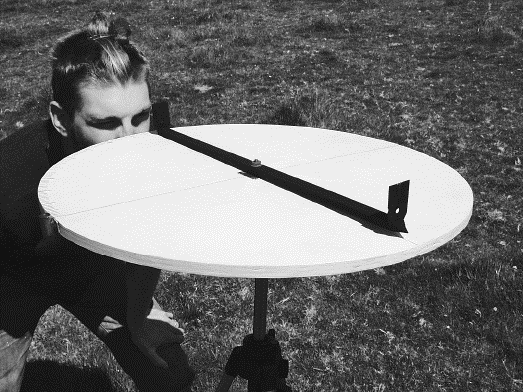
\includegraphics[height= 0.4\linewidth]{5a}
		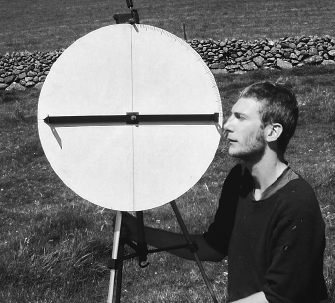
\includegraphics[height= 0.4\linewidth]{5b}
		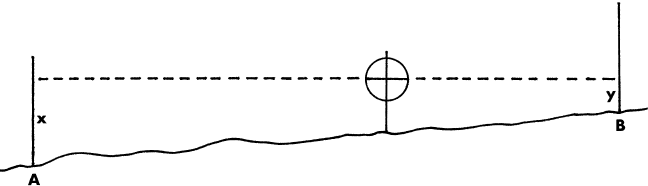
\includegraphics[width= 1\linewidth]{5c}
		\caption{\small\textit{\color{toanhocdoisong}Hình $5$. Trên: Dioptra trong mặt phẳng nằm ngang và mặt phẳng thẳng đứng. Dưới: Dùng dioptra xác định phương nằm ngang, qua đó đo được chênh lệch độ cao giữa hai điểm $A$ và $B$.}}
		\vspace*{-10pt}
	\end{figure}
	Về cơ bản, \textit{dioptra} gồm một thước ngắm trên một đĩa (gỗ hoặc kim loại). Thước ngắm có lỗ tròn hoặc khe hẹp giúp tăng độ chính xác so với chỉ ngắm bằng mắt thường qua các đầu cọc. Vạch trên đĩa vuông góc với thước cho phép xác định phương vuông góc. \textit{Dioptra} có thể được sử dụng trong mặt phẳng ngang cũng như trong mặt phẳng thẳng đứng vuông góc với mặt đất.
	\vskip 0.1cm
	Những tài liệu còn sót lại của Julius Africanus, một tác giả La Mã ở Jerusalem ở thế kỷ $3$, và một tác giả khuyết danh vào thế kỷ $10$ ở Byzantine (hậu duệ của đế quốc Đông La Mã) ghi chép về việc sử dụng \textit{dioptra} để đo khoảng cách và chiều cao. Đặc biệt, Julius Africanus mô tả cách sử dụng dioptra trong quân sự để đo chiều cao của tường thành địch. Tuy vậy, những ứng dụng này của \textit{dioptra} lại không xuất hiện trong các ghi chép có nguồn gốc ở phía Tây của đế quốc La Mã. Đây là một vấn đề hiện nay vẫn chưa thể giải thích rõ ràng. Một nguyên nhân có thể là do nguồn gốc Hy Lạp của \textit{dioptra} không được tiếp nhận tích cực ở nửa Tây của La Mã trong khi ở phía Đông, ảnh hưởng của văn minh Hy Lạp mạnh hơn (sau khi Đông La Mã trở thành Byzantine, tiếng Hy Lạp thay thế tiếng Latin thành ngôn ngữ chính thức).
	\vskip 0.1cm
	Nghiên cứu khảo cổ cũng cho thấy đồng hồ mặt trời xuất hiện trong bộ thiết bị của một nhà trắc địa La Mã cổ đại. Nó cho phép người ta xác định phương hướng vào ban ngày. Vào ban đêm, các chòm sao được dùng làm công cụ định hướng. Trong di tích nơi ở của một người làm trắc địa ở di chỉ Pompeii, có một ngôi nhà mà  sàn của nó được khảm trang trí câu chuyện về Orion, nhân vật thần thoại sau khi chết trở thành một chòm sao trên bầu trời. Chòm sao này có tác dụng quan trọng dùng để định vị các chòm sao khác. Không những cần các kỹ năng đo đạc trên mặt đất, người làm trắc địa thời La Mã còn phải có hiểu biết về bầu trời nữa!
	\begin{figure}[H]
		\vspace*{-5pt}
		\centering
		\captionsetup{labelformat= empty, justification=centering}
		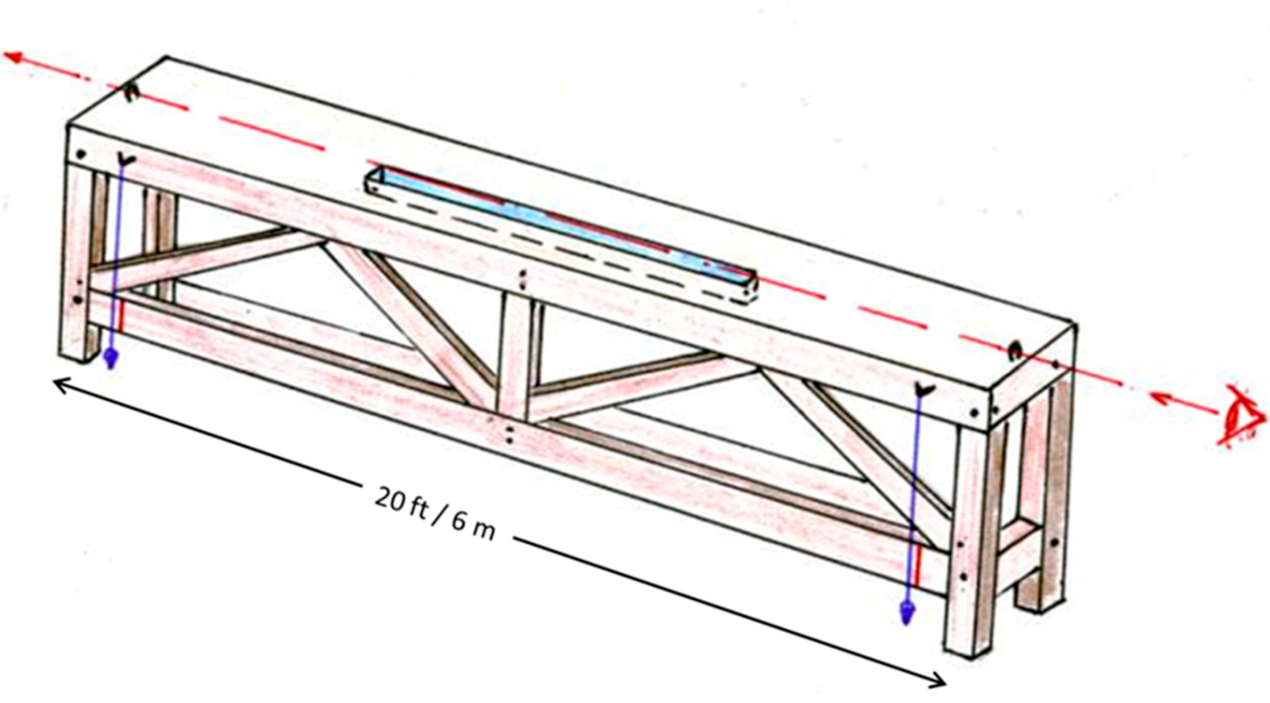
\includegraphics[width= 0.85\linewidth]{6a}
		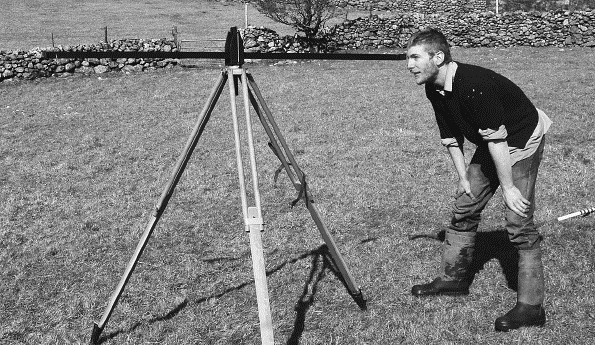
\includegraphics[width= 0.85\linewidth]{6}
		\caption{\small\textit{\color{toanhocdoisong}Hình $6$. Trên: Mô hình phục dựng lại chorobates. Dưới: Libra có cấu tạo là một thước ngắm dạng đòn cân dài có giá đỡ.}}
		\vspace*{-10pt}
	\end{figure}
	Một vấn đề trắc địa quan trọng khác là việc xác định phương nằm ngang. Đây là một yêu cầu thiết yếu khi người La Mã xây dựng các hệ thống dẫn nước dài nhiều cây số. Nhiều tài liệu hiện nay cho rằng người ta đã sử dụng thiết bị mang tên \textit{chorobates} có dạng một ghế băng dài với một máng khoét ở giữa có đổ nước. Khi mặt ghế hoàn toàn nằm ngang, mực nước sẽ ở đều cả hai bên máng. Tuy nhiên, về mặt kỹ thuật, độ chính xác của nó không cao và các thiết bị chính xác hơn nhiều như \textit{dioptra} và \textit{libra} có thể đã được sử dụng (Hình $6$). 
	\vskip 0.1cm
	Về mặt đo khoảng cách, ngoài dây thừng và gậy, người La Mã có một thiết bị khá thú vị là \textit{hodometer} có nguồn gốc Hy Lạp. Khi người sử dụng đẩy xe, trục bánh xe sẽ kéo theo các bánh răng bên trong xe chuyển động. Các bánh răng được tính toán sao cho khi xe đi được một dặm La Mã, một hòn sỏi sẽ chui qua lỗ ở trên xuống phía dưới và ta chỉ cần đếm số lượng hòn sỏi để biết đã đi được bao xa. Tuy khá phức tạp về mặt cơ khí, \textit{hodometer} không có độ chính xác cao do quá trình di chuyển khi đẩy xe giữa hai điểm trong thực tế thường gấp khúc chứ không phải đường thẳng.
	\begin{figure}[H]
		\vspace*{-5pt}
		\centering
		\captionsetup{labelformat= empty, justification=centering}
		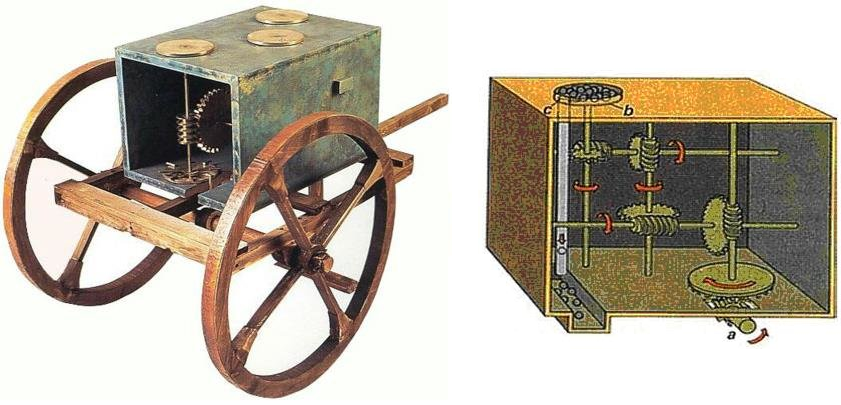
\includegraphics[width= 1\linewidth]{7}
		\caption{\small\textit{\color{toanhocdoisong}Hình $7$. Hodometer.}}
		\vspace*{-10pt}
	\end{figure}
	\textbf{\color{toanhocdoisong}Bài tập}
	\vskip 0.1cm
	Trong các bài tập trắc địa dưới đây, phương vuông góc có thể được xác định bằng \textit{groma} hoặc \textit{dioptra}.
	\vskip 0.1cm
	$\pmb{1.}$ \textit{Tìm khoảng cách giữa điểm $A$ (ở gần) và điểm $B$ (ở xa) mà không cần đi đến $B$.} 
	\vskip 0.1cm
	Phương pháp: Cắm cọc ở $\Gamma$  thẳng hàng với $A$ và $B$. Cắm cọc ở $E$ sao cho $\Gamma E$ vuông góc với $B\Gamma$. Trên $BE$, xác định $\Delta$ sao cho $A\Delta$ vuông góc với $B\Gamma$. Đo các khoảng cách $A\Delta$, $A\Gamma$, $E\Gamma$.
	\vskip 0.1cm 
	Hãy viết biểu thức của độ dài đoạn $AB$.
	\begin{figure}[H]
		\vspace*{-5pt}
		\centering
		\captionsetup{labelformat= empty, justification=centering}
		\begin{tikzpicture}[color=toanhocdoisong,scale=0.72, node font=\small]
			\draw  (0.,0.)-- (5.,0.);
			\draw  (5.,0.)-- (5.,3.);
			\draw  (5.,3.)-- (0.,0.);
			\draw  (3.,0.)-- (3.0176470588235293,1.8105882352941176);
			\draw [fill=white] (0.,0.) circle (1.5pt);
			\draw (-0.4,-0.09) node {$B$};
			\draw [fill=white] (5.,0.) circle (1.5pt);
			\draw (5.22,-0.5) node {$\Gamma$};
			\draw [fill=white] (5.,3.) circle (1.5pt);
			\draw (5.14,3.37) node {$E$};
			\draw [fill=white] (3.,0.) circle (1.5pt);
			\draw (2.96,-0.5) node {$A$};
			\draw [fill=white] (3.0176470588235293,1.8105882352941176) circle (1.5pt);
			\draw (3.03,2.32) node {$\Delta$};
		\end{tikzpicture}
		\vspace*{-10pt}
	\end{figure}
	$\pmb{2.}$ \textit{Đo chiều cao của bức tường $AB$ mà không đến $B$.} 
	\vskip 0.1cm
	Phương pháp: Cắm \textit{dioptra} tại $\Gamma$ và gióng thước ngắm đến $A$. Giữ nguyên thước ngắm và ngắm theo chiều ngược lại để xác định điểm $E$ trên mặt đất. Đo $\Gamma E$ và $\Gamma\Delta$ với $\Delta$ là tâm của đĩa tròn của \textit{dioptra}. Đo $EB$ theo phương pháp ở bài $1$.
	\vskip 0.1cm 
	Hãy viết biểu thức cho độ cao $AB$.  
	\begin{figure}[H]
		\vspace*{-5pt}
		\centering
		\captionsetup{labelformat= empty, justification=centering}
		\begin{tikzpicture}[color=toanhocdoisong, scale=0.72, node font=\small]
			\draw  (0.,4.)-- (0.,1.);
			\draw  (0.,1.)-- (5.,1.);
			\draw  (5.,1.)-- (0.,4.);
			\draw  (2.9970588235294118,2.201764705882353)-- (3.,1.);
			\draw  (2.9970588235294118,2.201764705882353) circle (0.3210460842858762cm);
			\draw  (2.9970588235294118,2.201764705882353)-- (2.996273103698748,2.5228098286916585);
				\draw [fill=white] (0.,4.) circle (1.5pt);
				\draw (-0.1,4.41) node {$A$};
				\draw [fill=white] (0.,1.) circle (1.5pt);
				\draw (-0.3,0.99) node {$B$};
				\draw [fill=white] (5.,1.) circle (1.5pt);
				\draw (5.34,0.99) node {$E$};
				\draw [fill=white] (3.,1.) circle (1.5pt);
				\draw (2.8,1.38) node {$\Gamma$};
				\draw [fill=white] (2.996273103698748,2.5228098286916585) circle (1.5pt);
				\draw (2.9,2.9) node {$\Delta$};
		\end{tikzpicture}
		\vspace*{-10pt}
	\end{figure}
	$\pmb{3.}$ $a)$ \textit{Đo khoảng cách giữa hai điểm $A$ và $B$ có thể nhìn thấy nhưng không thể đến được.}
	\vskip 0.1cm 
	Phương pháp: Sử dụng phương pháp ở bài $1$ để đo các khoảng cách $\Gamma A$ và $\Gamma B$ khi đứng ở $\Gamma$. Gióng các cọc tại $\Delta$ và $E$ sao cho $\dfrac{\Gamma\Delta}{\Gamma E}=\dfrac{\Gamma A}{\Gamma B}$. Đo độ dài $\Delta E$.
	\vskip 0.1cm 
	Hãy viết biểu thức cho độ dài $AB$.
	\begin{figure}[H]
		\vspace*{-5pt}
		\centering
		\captionsetup{labelformat= empty, justification=centering}
		\begin{tikzpicture}[color=toanhocdoisong, scale=0.72, node font=\small]
			\draw  (2.,2.)-- (0.,5.);
			\draw  (-4.5,2.)-- (2.,2.);
			\draw  (-2.076923076923077,3.6153846153846154)-- (-1.,2.);
			\draw  (-4.5,2.)-- (0.,5.);
			
			\draw [fill=white] (2.,2.) circle (1.5pt);
			\draw (2.3,1.93) node {$B$};
			\draw [fill=white] (0.,5.) circle (1.5pt);
			\draw (0.14,5.37) node {$A$};
			\draw [fill=white] (-4.5,2.) circle (1.5pt);
			\draw (-4.9,1.93) node {$\Gamma$};
			\draw [fill=white] (-1.,2.) circle (1.5pt);
			\draw (-0.92,1.55) node {$E$};
			\draw [fill=white] (-2.076923076923077,3.6153846153846154) circle (1.5pt);
			\draw (-2.2,3.99) node {$\Delta$};
		\end{tikzpicture}
		\vspace*{-10pt}
	\end{figure}
	$b)$ Hãy chứng minh $\Delta E$ song song với $AB$ để chỉ ra rằng phương pháp trên cũng cho phép xác định phương song song với với đường thẳng đi qua hai điểm ở xa.
	\vskip 0.1cm
	$\pmb{2.}$ \textbf{\color{toanhocdoisong}Trắc địa trên khoảng cách lớn}
	\vskip 0.1cm
	Trong việc xây dựng các con đường nối hai địa điểm, trừ khi có chướng ngại vật, người ta luôn hướng đến việc đi theo đường thẳng thay vì đường cong. Việc xác định đường thẳng trên thực địa là một vấn đề quan trọng mà người làm trắc địa La Mã cần phải giải quyết. Các công cụ gióng hàng nêu ở phần trên có thể giúp gióng hàng ở khoảng cách ngắn từ vài trăm mét đến vài km. Với những khoảng cách lớn hơn, vấn đề bắt đầu trở nên phức tạp hơn.
	\begin{figure}[H]
		\vspace*{-5pt}
		\centering
		\captionsetup{labelformat= empty, justification=centering}
		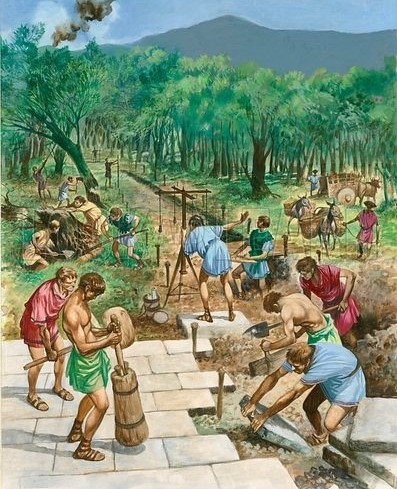
\includegraphics[height= 0.8\linewidth]{8}
		\caption{\small\textit{\color{toanhocdoisong}Hình $8$. Minh họa về xây dựng đường thời La Mã (Peter Jackson). Kỹ thuật viên ở giữa đang gióng hàng với một người cầm cọc và một cột khói ở địa điểm ở phía xa.}}
		\vspace*{-10pt}
	\end{figure}
	Nếu không thể nhìn thấy điểm kết thúc từ điểm bắt đầu con đường, người ta có thể đốt lửa tạo cột khói để tiến hành gióng hàng. Tuy nhiên, với những khoảng cách lớn hơn nữa, công việc cũng trở nên phức tạp hơn nhiều. 
	\begin{figure}[H]
		\vspace*{-5pt}
		\centering
		\captionsetup{labelformat= empty, justification=centering}
		\begin{tikzpicture}[scale=0.7, color=toanhocdoisong]
			\draw [dashed] (0,0) -- (10,0);
			\draw [fill= black] (0,0) circle (3pt);
			\draw [fill= white] (2,0.5) circle (3pt);
			\draw [fill= white] (4,-0.5) circle (3pt);
			\draw [fill= white] (6,0.5) circle (3pt);
			\draw [fill= white] (8,-0.5) circle (3pt);
			\draw [fill= black] (10,0) circle (3pt);
		\end{tikzpicture}
		\caption{\small\textit{\color{toanhocdoisong}Hình $9$. Gióng hàng bằng xấp xỉ liên tiếp. Các cọc màu trắng sẽ được di chuyển đến lúc nào tất cả chúng đều thẳng hàng với hai vị trí đầu và cuối (hai cọc màu đen).}}
		\vspace*{-10pt}
	\end{figure}
	Một giả thuyết được đưa ra là đầu tiên người ta cắm một số cọc đánh dấu xấp xỉ, mỗi cọc chỉ có thể quan sát được một cọc phía trước và một cọc phía sau. Do không xác định chính xác được đường thẳng nối điểm đầu và điểm cuối trên thực địa, các cọc sẽ được di chuyển bằng cách thử dần cho đến khi nào tất cả các cọc đều thẳng hàng (kể cả cọc cố định ở điểm đầu và điểm cuối). Phương pháp xấp xỉ liên tiếp này tuy có thể thực hiện được nhưng sẽ mất rất nhiều thời gian và công sức lao động.
	\vskip 0.1cm
	Một giả thuyết khác là các nhà trắc địa La Mã đã sử dụng cách đo khoảng cách của Heron. Chọn một phương làm phương cơ sở (ví dụ phương Đông Tây). Sau đó ta chỉ di chuyển theo phương này hoặc phương vuông góc với nó. Đến mỗi điểm đánh dấu (ví dụ ngọn đồi), người ta ghi lại tổng độ dài đã đi theo mỗi phương. Từ đó, một bản đồ giống với lưới tọa độ có thể được vẽ ra. Các vị trí trên đường đi sẽ được thiết lập theo độ lệch của nó so với đường gấp khúc nối các điểm đánh dấu.
	\begin{figure}[H]
		\vspace*{-5pt}
		\centering
		\captionsetup{labelformat= empty, justification=centering}
		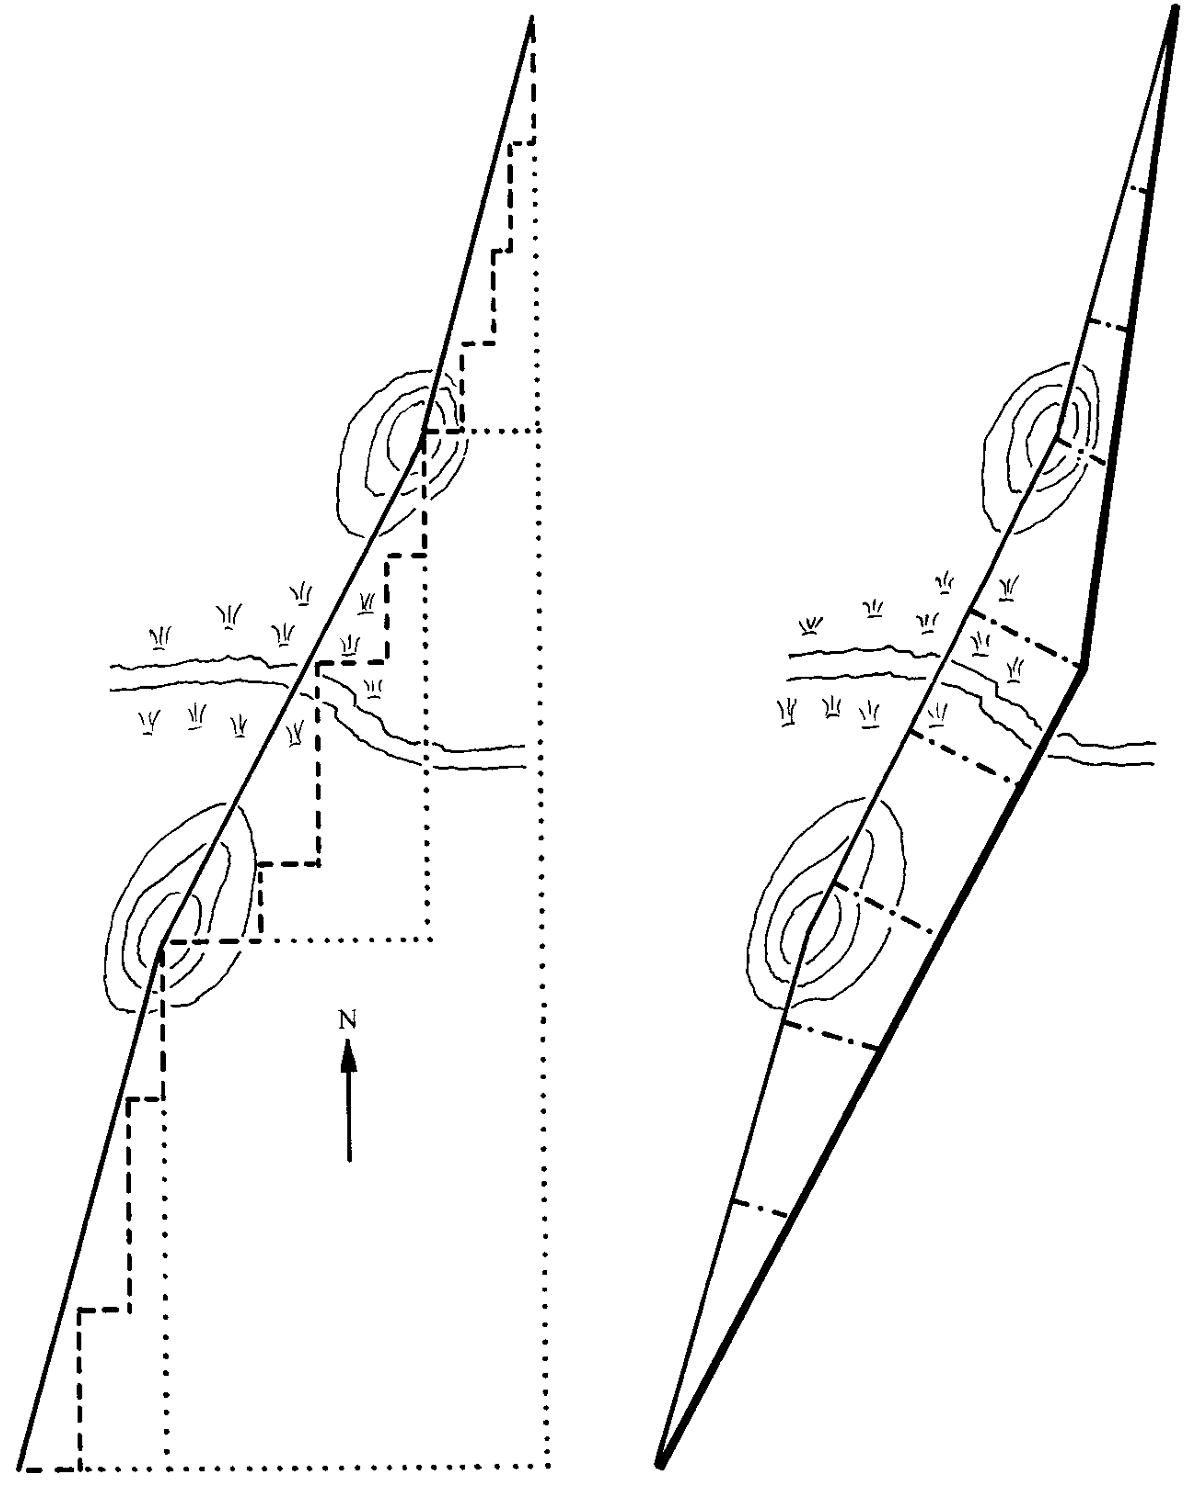
\includegraphics[height= 0.7\linewidth]{10}
		\caption{\small\textit{\color{toanhocdoisong}Hình $10$. Xác định vị trí bằng cách di chuyển theo hai phương vuông góc.}}
		\vspace*{-10pt}
	\end{figure}
	Trong một phiên bản khác của phương pháp này, việc trắc địa sẽ không có thao tác vẽ bản đồ mà được hoàn toàn tiến hành trên thực địa. Ứng với mỗi điểm đánh dấu, người ta đo khoảng cách đến điểm đánh dấu trước nó bằng các phương pháp đo trắc địa. Góc của đường nối cũng được xác định bằng góc so với phương Bắc – Nam. Góc ở giai đoạn lịch sử này không biểu diễn bằng độ mà được biểu diễn bằng tỷ lệ giữa hai cạnh góc vuông – tức là $\tan$ của góc. Khoảng cách và góc giữa điểm đầu và điểm cuối có thể được xác định bằng cách tính các cạnh của tam giác vuông theo định lý Pythagoras và tam giác đồng dạng. Nhờ đó, có thể tiến hành gióng hàng để xác định đường thẳng nối hai điểm đã cho.
	\begin{figure}[H]
		\vspace*{-5pt}
		\centering
		\captionsetup{labelformat= empty, justification=centering}
		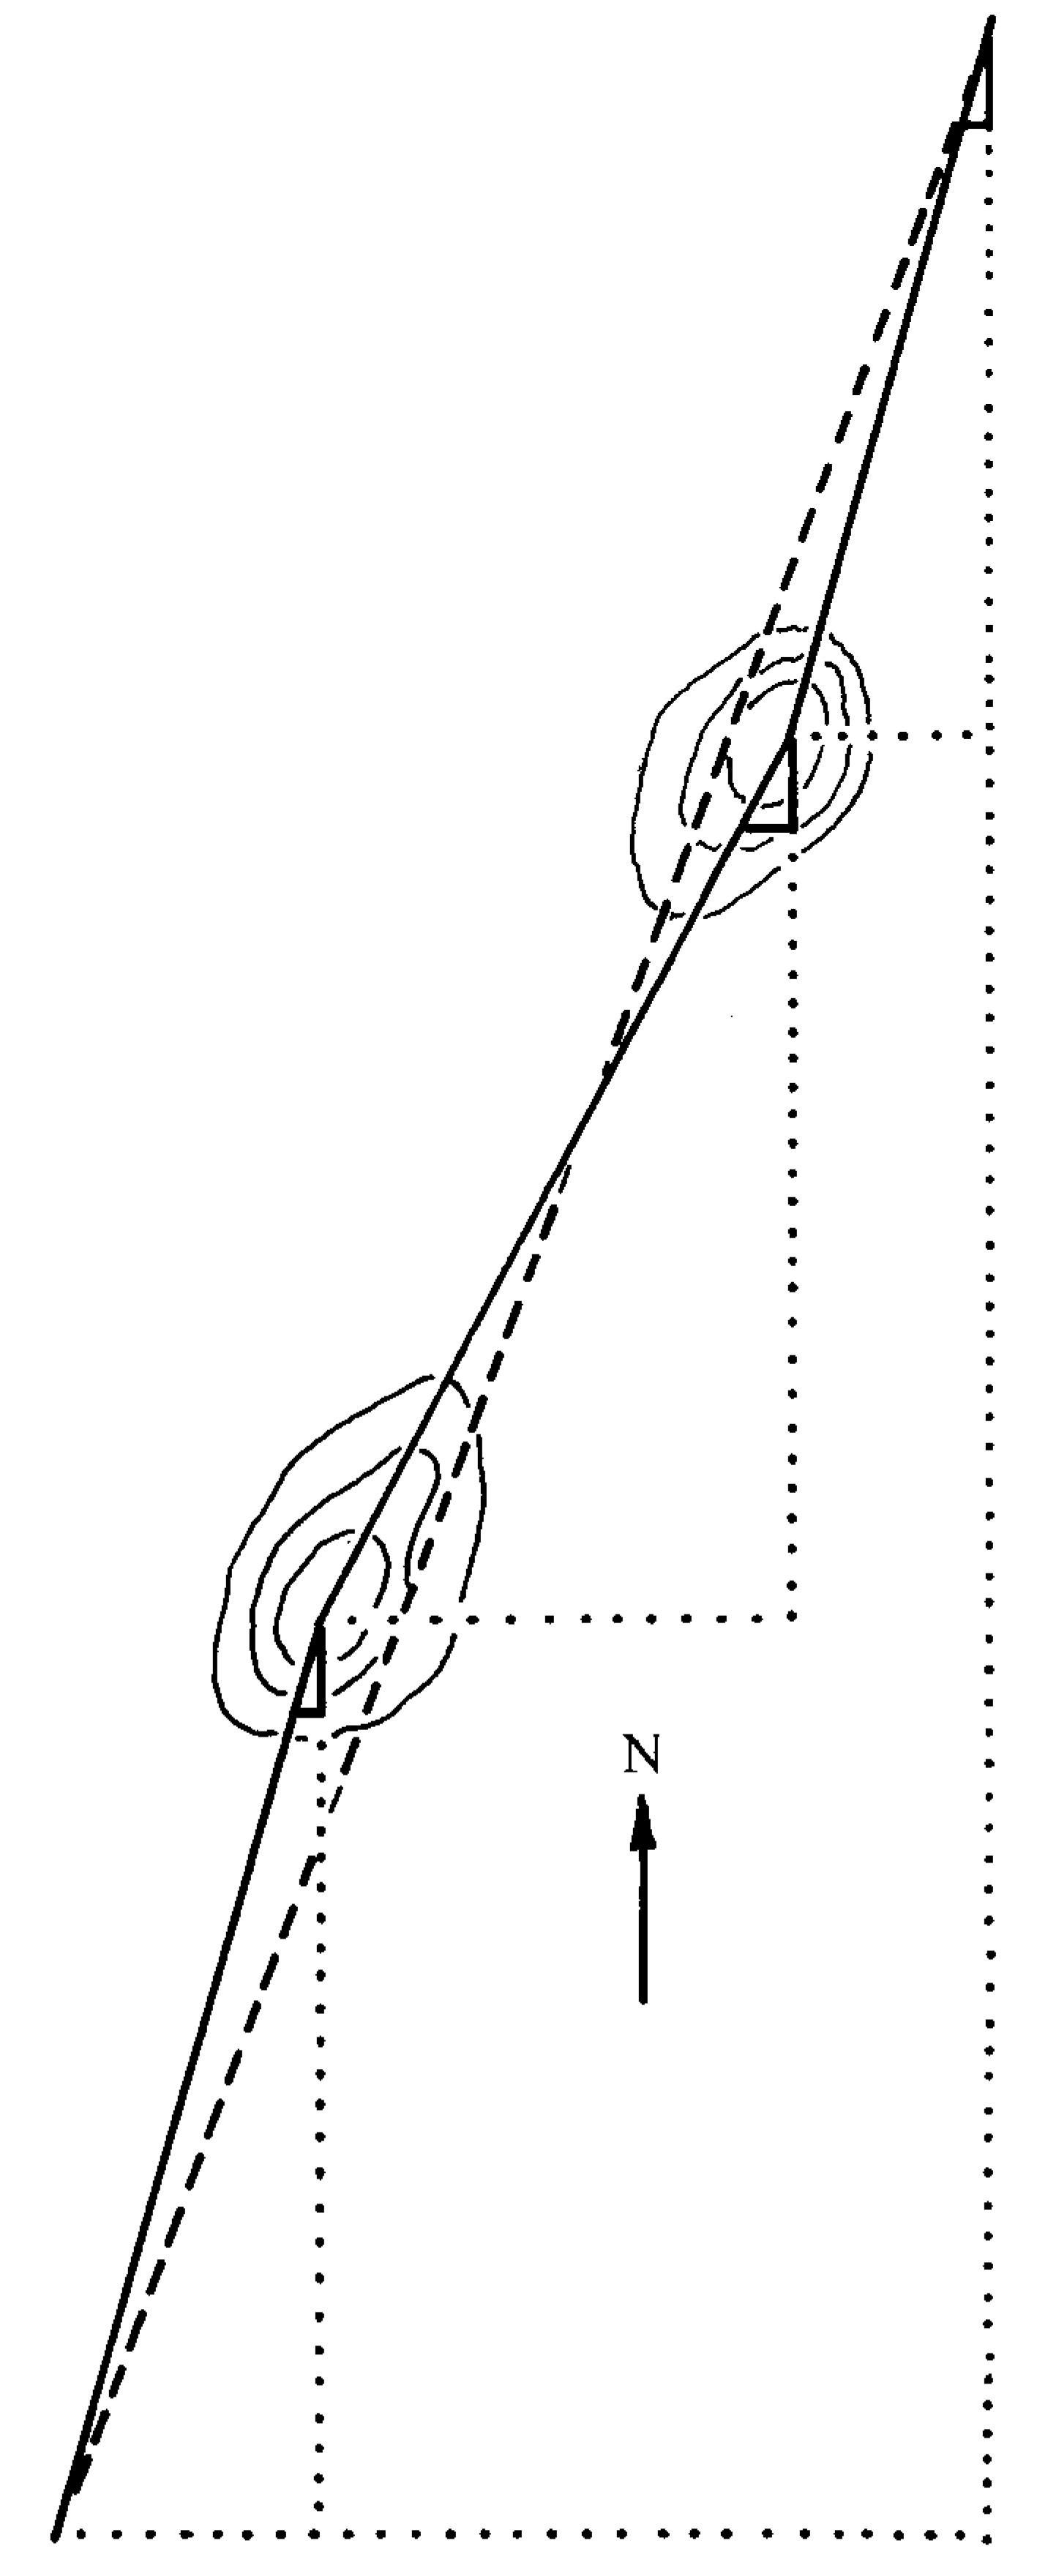
\includegraphics[height= 0.7\linewidth]{11}
		\caption{\small\textit{\color{toanhocdoisong}Hình $11$. Xác định vị trí theo khoảng cách và góc.}}
		\vspace*{-10pt}
	\end{figure}
	Một giả thuyết khác được nhà nghiên cứu M. Lewis đưa ra là việc gióng hàng trên khoảng cách lớn bằng dựng hình. Theo đó, người ta tiến hành gióng hàng theo một phương $AX$ mang tính ước lượng và xác định xem $B$ nằm ở nửa mặt phẳng nào so với $AX$, sau đó tiến hành gióng hàng theo hai phương $AY$ và $AZ$ sao cho $B$ nằm trong góc tạo bởi hai tia này. Khi đến đủ gần để chắc chắn rằng $B$ đúng là như vậy, các đường song song với $AY$ và $AZ$ được gióng từ $B$ (bằng cách sử dụng góc tạo với phương Bắc – Nam theo dạng tỷ lệ hai cạnh góc vuông) để tạo hình bình hành $ACBD$. Sau khi đo khoảng cách $CD$, trung điểm $E$ của đoạn thẳng này có thể được xác định. Điểm $E$ đồng thời cũng là trung điểm của $AB$. Các trung điểm của $AE$ và $EB$ có thể được tìm ra một cách tương tự. Quá trình xác định các trung điểm được lặp lại cho đến khi tất cả vị trí có thể được gióng hàng bằng các cọc liên tiếp sử dụng \textit{groma} hoặc \textit{dioptra}. 
	\vskip 0.1cm
	Một điểm đáng chú ý là một số con đường La Mã không được xây dựng hoàn toàn từ số không mà có mục đích nối các trung tâm dân cư đã có sẵn từ trước khi người La Mã đặt chân đến. Những con đường nối các địa điểm này dần hình thành theo lịch sử do hoạt động giao thông của con người cũng như việc chăn thả gia súc. Các đàn gia súc thường đi theo đường thẳng giữa các điểm có nhiều cỏ và nguồn nước -- đây cũng là các điểm mà dân cư thường tụ tập. Do đó công việc trắc địa có những lúc được tiến hành một cách dễ dàng hơn dựa trên việc nắn thẳng lại các tuyến đường có sẵn.
		\begin{figure}[H]
		\vspace*{-10pt}
		\centering
		\captionsetup{labelformat= empty, justification=centering}
		\begin{tikzpicture}[toanhocdoisong, scale=0.7, node font=\small]
			\draw  (-4.,2.)-- (2.06,2.18);
			\draw  (2.,4.)-- (-4.,2.);
			\draw  (-4.,2.)-- (2.,0.);
			\draw[dashed]  (-4.,2.)-- (2.,1.);
			\draw[-stealth]  (-3.38,2.6)-- (-3.38,3.54);
			\draw  (-1.245454545454544,2.0818181818181816)-- (2.,1.);
			\draw  (2.,1.)-- (-0.7545454545454544,0.9181818181818181);
			\draw[dashed]  (-1.245454545454544,2.0818181818181816)-- (-0.7545454545454544,0.9181818181818181);
			%			\draw [fill=white] (-4.,2.) circle (1.5pt);
			\draw (-3.86,2.37) node {$A$};
			%			\draw [fill=white] (2.06,2.18) circle (1.5pt);
			\draw (2.2,2.55) node {$Y$};
			%			\draw [fill=white] (2.,4.) circle (1.5pt);
			\draw (2.14,4.37) node {$X$};
			%			\draw [fill=white] (2.,0.) circle (1.5pt);
			\draw (2.14,0.37) node {$Z$};
			%			\draw [fill=white] (2.,1.) circle (1.5pt);
			\draw (2.14,1.37) node {$B$};
			%			\draw [fill=white] (-1.,1.5) circle (1.5pt);
			\draw (-0.86,1.75) node {$E$};
			%			\draw [fill=white] (-1.245454545454544,2.0818181818181816) circle (1.5pt);
			\draw (-1.1,2.41) node {$C$};
			%			\draw [fill=white] (-0.7545454545454544,0.9181818181818181) circle (1.5pt);
			\draw (-0.69,0.49) node {$D$};
			%			\draw [fill=white] (-3.38,3.54) circle (1.5pt);
			\draw (-3.4,3.95) node {$N$};
			%			\draw[color=black] (-1.24,1.55) node {$p$};
		\end{tikzpicture}
		\caption{\small\textit{\color{toanhocdoisong}Hình $12$. Trắc địa bằng dựng hình.}}
		\vspace*{-10pt}
	\end{figure}
	Có thể nói, phương pháp gióng hàng trên khoảng cách lớn mà người La Mã đã sử dụng vẫn là một vấn đề mở với các hướng nghiên cứu khác nhau và khó có thể kết luận được một cách dễ dàng với lượng chứng cứ ít ỏi còn lại.
	\vskip 0.1cm
	$\pmb{3.}$ \textbf{\color{toanhocdoisong}Vai trò của trắc địa trong kinh tế xã hội La Mã}
	\begin{figure}[H]
		\vspace*{-5pt}
		\centering
		\captionsetup{labelformat= empty, justification=centering}
		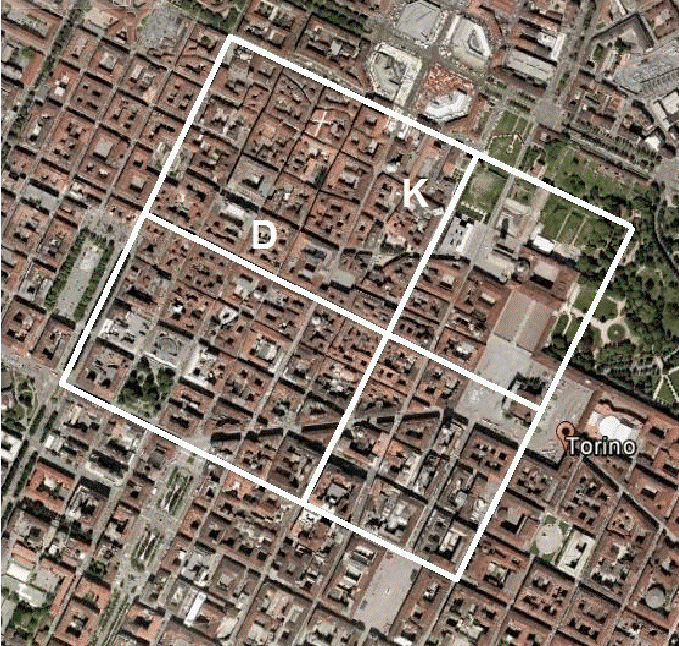
\includegraphics[height= 0.7\linewidth]{13}
		\caption{\small\textit{\color{toanhocdoisong}Hình $13$. Lưới ô vuông của một di tích La Mã.}}
		\vspace*{-10pt}
	\end{figure}
	Trắc địa có dấu ấn quan trọng trong việc quy hoạch các khu vực đô thị cũng như đất nông nghiệp ở La Mã. Các khu vực này sẽ được chia theo các lưới ô vuông dọc theo các trục đường chính trước khi xây dựng. Những người làm trắc địa không chỉ tiến hành đo đạc mà còn phải có hiểu biết về pháp luật để tiến hành giải quyết các tranh chấp khiếu kiện về đất đai.
	\begin{figure}[H]
		\vspace*{-5pt}
		\centering
		\captionsetup{labelformat= empty, justification=centering}
		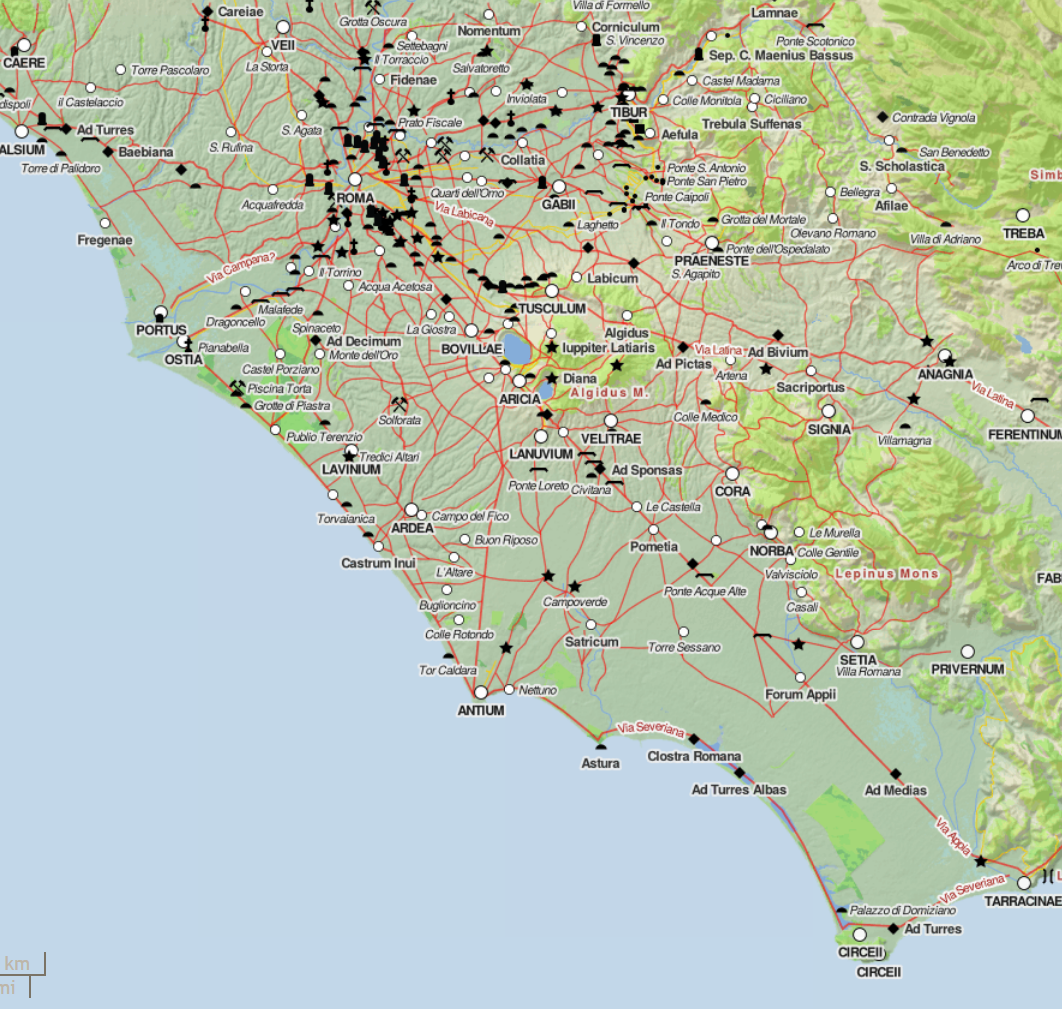
\includegraphics[height= 0.7\linewidth]{14}
		\caption{\small\textit{\color{toanhocdoisong}Hình $14$. Hệ thống đường giao thông xung quanh Rome thời La Mã cổ đại.}}
		\vspace*{-10pt}
	\end{figure}
	Hệ thống đường giao thông La Mã cũng mang đậm dấu ấn của những nhà trắc địa. Mạng lưới đường bộ trải khắp đế quốc được thiết kế với mức độ thẳng nhất mà địa hình cho phép, giúp đảm bảo tốc độ vận chuyển nhanh chóng nhất cho các hoạt động kinh tế cũng như quân sự của một đế quốc khổng lồ. Nhiều đoạn đường trong hệ thống này có độ dài thẳng tắp từ vài chục đến hàng trăm km.
	
	\begin{figure}[H]
		\vspace*{-5pt}
		\centering
		\captionsetup{labelformat= empty, justification=centering}
		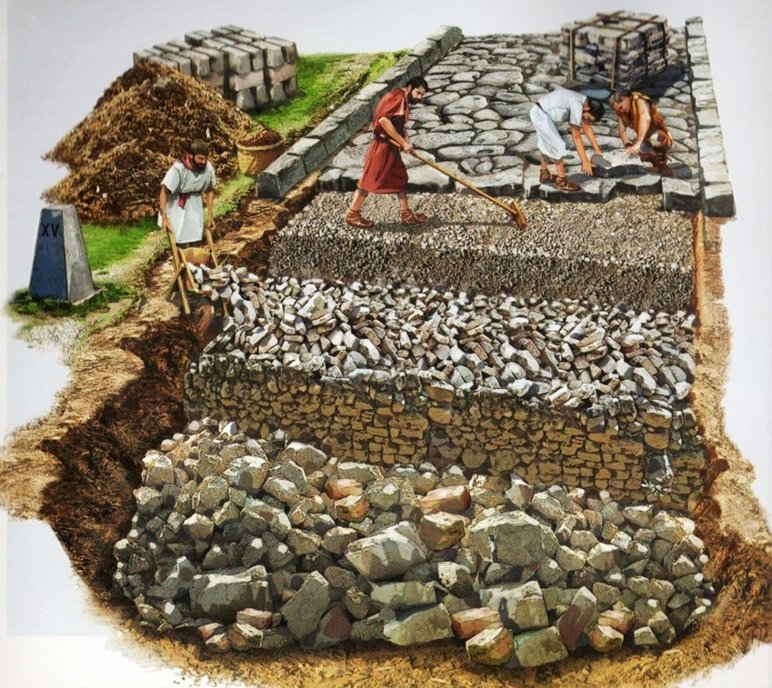
\includegraphics[height= 0.36\linewidth]{15a}
		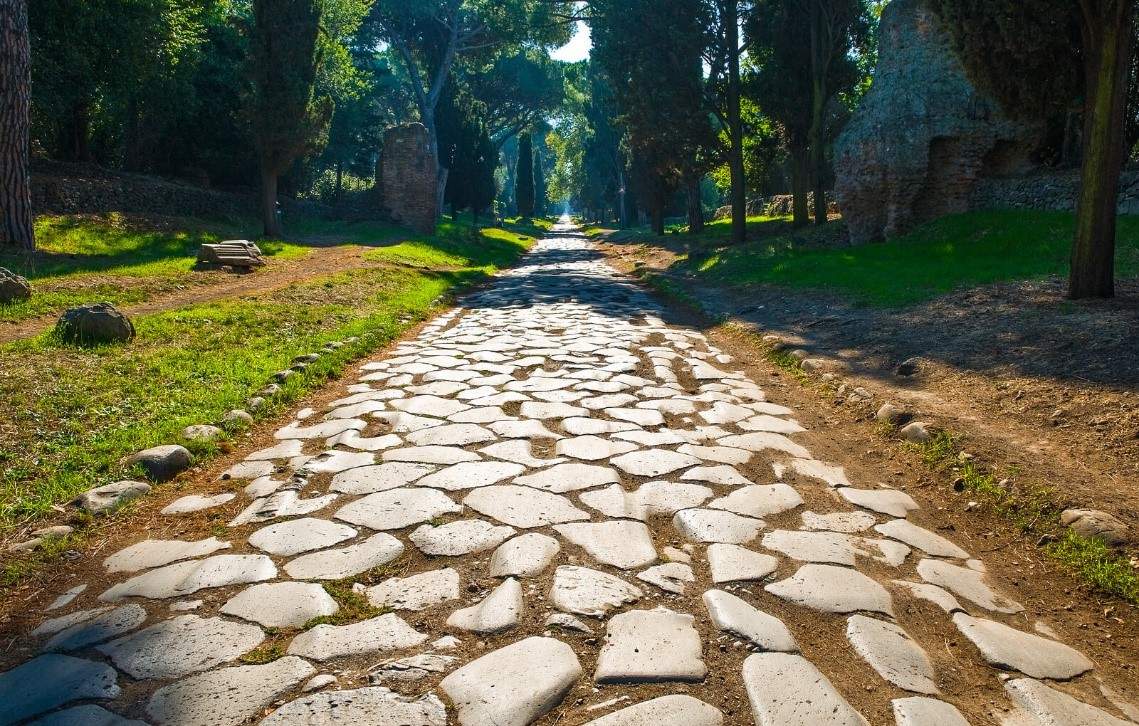
\includegraphics[height= 0.36\linewidth]{15b}
		\caption{\small\textit{\color{toanhocdoisong}Hình $15$. Trái: Đường bộ thời La Mã được xây dựng công phu với nhiều lớp vật liệu khác nhau. Phải: Một con đường thời La Mã vẫn tồn tại đến ngày nay.}}
		\vspace*{-10pt}
	\end{figure}
	Các con đường thời La Mã được xây dựng một cách công phu với nhiều lớp vật liệu khác nhau đảm bảo tính bền chắc cũng như thoát nước tốt. Nhiều đoạn vẫn còn tồn tại hàng nghìn năm cho đến ngày nay. Dọc theo các con đường là những cột mốc đánh dấu khoảng cách tính từ cột mốc số không, được đặt tại Rome -- đầu não của toàn bộ đế quốc. Đây cũng là nguồn gốc của câu nói ``Mọi con đường đều dẫn đến Rome".
	\vskip 0.1cm
	Một thành tựu đáng chú ý khác của trắc địa thời La Mã là việc xây dựng các hệ thống đường ống dẫn nước (\textit{aqueduct}). Để cung cấp nước sinh hoạt cho khu vực đô thị, người ta phải dẫn nguồn nước từ các vị trí cao như suối hay hồ trên núi theo hệ thống đường dẫn có thể lên đến hàng chục km. Do chưa biết đến hiện tượng bình thông nhau, toàn bộ hệ thống ống dẫn được xây dựng với độ dốc hướng xuống. Trên những quãng đường xa như vậy, độ dốc này phải rất nhỏ, trung bình khoảng một trên vài nghìn, ở một số đoạn độ dốc chỉ là $1/20000$. Có những đoạn phải được đào theo những đường hầm xuyên núi. Những hệ thống dẫn nước này cho thấy độ chính xác cao trong việc tiến hành trắc địa và đo đạc khi xây dựng. Đồng thời, chúng cũng là biểu tượng cho sự thịnh vượng và phồn vinh của đế quốc.
	\begin{figure}[H]
		\vspace*{-5pt}
		\centering
		\captionsetup{labelformat= empty, justification=centering}
		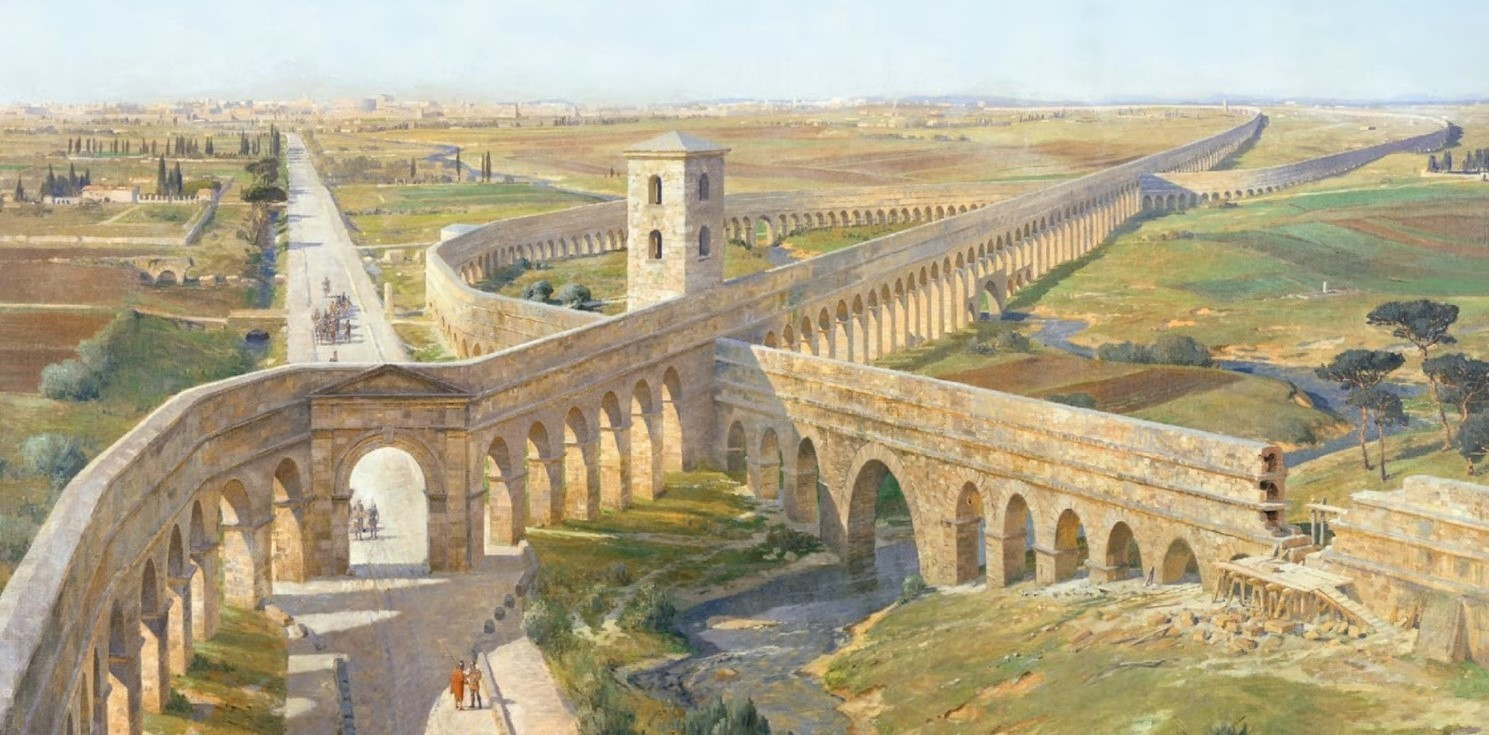
\includegraphics[width= 1\linewidth]{16}
		\caption{\small\textit{\color{toanhocdoisong}Hình $16$. Hệ thống dẫn nước gần thành Rome}}
		\vspace*{-10pt}
	\end{figure}
	Có thể nói, tuy kế thừa nhiều công cụ và kiến thức trắc địa từ các nền văn minh khác nhau như Ai Cập, Babylon, Hy Lạp,  người La Mã đã thể hiện sự vượt trội hơn hẳn trong việc ứng dụng vào thực tế xã hội, với nhiều thành quả đã được phát hiện và nghiên cứu.
	\vskip 0.1cm
	\textbf{\color{toanhocdoisong}Tài liệu tham khảo}
	\vskip 0.1cm
	[$1$] Jean--Pierre Adam. ($1994$). \textit{Roman building : materials and techniques}. Batsford.
	\vskip 0.1cm
	[$2$] Lewis, M. J. T. ($2001$). \textit{Surveying instruments of Greece and Rome}. Cambridge University Press.
	\vskip 0.1cm
	[$3$] Talbert, R. J. A. ($2012$). \textit{Ancient perspectives : maps and their place in Mesopotamia, Egypt, Greece $\&$ Rome}. The University Of Chicago Press.
\end{multicols}